% GUIDA VELOCE:
% --------------------------------------------------------------------
% X INIZIA UN UNOVO CAPITOLO:
% \chapter{??? NOME CAPITOLO}}
% 	\section{ ?? }
% 		\subsection{ ?? }
%
% --------------------------------------------------------------------
% PAROLA CONTENUTA NEL GLOSSARIO:
% scrivere la parola seguita da $^g$
% esempio: User$^g$
%
% --------------------------------------------------------------------
% PER ANDARE A CAPO SENZA RIENTRO INSERIRE:
% \\
%
% --------------------------------------------------------------------

% GRASSETO:
% \textbf{parola}
%
% --------------------------------------------------------------------
% CORSIVO:
% \emph{parola}

% --------------------------------------------------------------------
% PER SCRIVERE IN ROSSO:
% \red{parola}
%
% --------------------------------------------------------------------
% PER SCRIVERE TRA VIRGOLETTE
% ''parola''
%
% --------------------------------------------------------------------
% PER EVITARE IL RIENTRO AUTOMATICO DI UN CAPOVERSO:
% \noindent testo....
%
% --------------------------------------------------------------------

% PER SCRIVERE CARATTERI PARTICOLARI COME: { } _  ecc.. SCRIVERLI PRECEDUTI DA \
% ES: \{  \_
%
% --------------------------------------------------------------------
% X INSERIRE UN LINK:
% \url{http://www.math.unipd.it/~tullio/IS-1/2011/Progetto/C3.pdf}
%
% --------------------------------------------------------------------
% PER COMMENTARE INTERE PARTI:
% \comment{ comment }
%
% --------------------------------------------------------------------
% PER SCRIVERE NOTE DURANTE IL TESTO:
% parola \footnote{ note riguardanti la parola }
%
% --------------------------------------------------------------------
% PER SCRIVERE CODICE SORGENTE:
%
% \lstset{language=c++,
% stringstyle=\color{blue}\textrm,
% commentstyle=\rmfamily, numbers= none}

% \begin{lstlisting}
%  CODICE
% \end{lstlisting}
%
% --------------------------------------------------------------------
% !!!!!!!!     PER COSE + COMPLESSE VEDI:     !!!!!!!!!!!!!!!!!!!!!!!
% !!!!!!!!    PMAC/latex/GUIDA LATEX!!!.tex   !!!!!!!!!!!!!!!!!!!!!!!

% per tutto il resto chiedi a lory prima di fare/scrivere cazzate !!!!!!!!!!


\documentclass[10pt,a4paper]{article}

\usepackage[italian]{babel} 
\usepackage[T1]{fontenc} 
\usepackage[utf8x]{inputenc} % uso utf8x xk x linux, mentre latin1 è per windows
\usepackage{lmodern} %insieme di font molto completo consigliato da LatexFacile pg13 in basso
\usepackage{microtype} %migliora riempimento delle righe. vedi LatexImpaziente pg41
%attiva il rientro di ogni prima riga di ogni sezione: capitolo,paragrafo ecc. vd LatexImpaziente pg41
\usepackage{indentfirst}
\usepackage{graphicx} % per inseire immagini
\usepackage[usenames,dvipsnames]{xcolor}
\usepackage{lastpage} %serve per poter scrivere page 1 of N
% setta i bordi della pagina: dx e sx 3.2cm di rientro + nel lato di rilagatura rientra di altri 0mm
\usepackage[a4paper,top=3cm,bottom=3cm,left=3.2cm,right=3.2cm, bindingoffset=0mm]{geometry}
\usepackage{listings} % per inserire codice sorgente
\usepackage{float}  % per gestire oggetti flottanti ( es immagini tabelle posizionebili con "H" che forza il posizionamento nel punto specifico

% serve per creare tabelle lunghe + di una pagina con \begin{longtable} (vd Tabelle.pdf pg11-12)
\usepackage{longtable} 

\usepackage{fancyhdr} % per impostare lo stile della pagina più personalizzato, + fancyhdr ( per regolare testatina e piè di pagina ) vedi itfancyhrd

\usepackage{array} % m nei tabular

\pagestyle{fancy}
% settaggi di pagestyle(fancy)
\lhead{
\includegraphics[scale=0.20]{SevenFold_small}}
%\chead{}
\rhead{\textbf{{%
\NomeDocumento\\ Data: \DataRilascio \\ e-mail: \mail{sevenfold@palomino.it}}}}
\lfoot{\NomeDocumento}
\cfoot{}
\rfoot{ \textbf \thepage\ di \pageref{LastPage}}
\renewcommand{\footrulewidth}{0.4pt}

%ridefinisco il plain per cosare l'indice (a questo punto si potrebbe lasciare tutto il documento in plain
\fancypagestyle{plain}{
\lhead{
\includegraphics[scale=0.20]{SevenFold_small}}
%\chead{}
\rhead{\textbf{{%
\NomeDocumento\\ Data: \DataRilascio \\ e-mail: \mail{sevenfold@palomino.it}}}}
\lfoot{\NomeDocumento}
\cfoot{}
\rfoot{ \textbf \thepage\ di \pageref{LastPage}}
\renewcommand{\footrulewidth}{0.4pt}
}

% da ultimo:
\usepackage{hyperref} %x l'interpretazione di indirizzi o link ipertestuali (vd LatexImpaziente pg47 )
\hypersetup{backref, colorlinks=true, linkcolor=black, urlcolor=black}

\usepackage{url} % x l'interpretazioni di internet o link ipertestuali (vd LatexImpaziente pg47 )
%\UrlFont{color =blue}
%\urlstyle{helvetic}

% Define a new 'leo' style for the package that will use a smaller font.
\makeatletter
\def\url@leostyle{%
  \@ifundefined{selectfont}{\def\UrlFont{\sf}}{\def\UrlFont{\small\ttfamily}}}
\makeatother
%% Now actually use the newly defined style.
\urlstyle{leo}


\newcommand{\mail}[1]{\textcolor{Black}{ \texttt{#1}}} %per interpretare mail (vd LatexImpaziente pg47 )
\newcommand{\cambiaFont}[2]{{\fontencoding{T1}\fontfamily{#1}\selectfont#2}}
\newcommand{\red}[1]{\textcolor{red}{#1}} % per scrivere testo in rosso
\newcommand{\comment}[1]{} % per inserire commenti

% per inserire una nuova lettera nella sezione Glossario
\newcommand{\newLetter}[1]{
\vspace{0.8cm}
\hspace{0.3cm}
\noindent{ \Large{ \textbf{\textcolor{blue}{#1}} } }

\noindent{\color{gray} \line(1,0){415} }\\
%\hspace{0.5cm}
}

\newcommand{\newWord}[1]{\noindent\textbf{\\#1}\\}



% INSERIRE QUI IL NOME DEL DOCUMENTO SEGUITO DA UNO SPAZIO
% ( così il nome si imposta in automatico nelle varie ricorrenze standard)
\newcommand{\NomeDocumento}{Manuale Utente: \emph{Mobile-user \underline{Android} }}

% INSERIRE QUI LA DATA DELLA VERSIONE DEL RILASCIO
\newcommand{\DataRilascio}{ 2012/09/19 }

% INSERISCI LA VERSIONE ATTUALE
\newcommand{\VersioneAttuale}{v2.0.0}

% INSERIRE QUI L'ACRONIMO DEL DOCUMENTO. ESEMPIO: Analisi Dei Requisiti = AR
% Quando inserite l'acronimo qui, dovete rinominare i file presenti nella cartella
% del tipo '??-cap1-NomeCapitolo.tex' sostituendo i '??' con l'acronimo scelto!!
\newcommand{\AcronimoDocumento}{??}

\begin{document}


% --------------------------------------------------------------------

% TITOLO ( 1° pagina)

\vspace*{2.5cm}
\begin{center}

%\cambiaFont{Cyklop}{Sevenfold}
%\cambiaFont{fve}{\Huge{Sevenfold}}

\includegraphics[scale=0.35]{SevenFold_big}

\vspace{2cm}

\cambiaFont{fve}{\Huge{\NomeDocumento}}\\
\vspace*{1cm}


\end{center}


% --------------------------------------------------------------------

\vspace*{2cm}
\begin{center}

\begin{tabular}{ r | l }
\multicolumn{2}{c}{\textbf{\huge{Informazioni sul documento}} }\\
\hline
\rule[-1.5mm]{0mm}{0.7cm}
\textbf{Titolo documento} & \NomeDocumento\\
\rule[-1.5mm]{0mm}{0.5cm}
\textbf{Data creazione}& 2012/09/19\\
\rule[-1.5mm]{0mm}{0.5cm}
\textbf{Distribuito da}& Gruppo SevenFold\\
\rule[-1.5mm]{0mm}{0.5cm}
\textbf{Destinato a}&Prof. Ghiraldo Filippo\\
&Gruppo Sevenfold\\

\end{tabular}

\end{center}


% --------------------------------------------------------------------

% SOMMARIO ( 2° pagina)

\newpage

\vspace*{0.5cm} % il vertical space va preceduto da una riga vuota!!!
\begin{center}

\textbf{{\huge{Sommario}}}

\vspace*{0.2cm} % il vertical space va preceduto da una riga vuota!!!

Questo documento ha lo scopo di descrivere il corretto utilizzo dell'applicazione Woty$^g$ inerentemente alle funzionalità del \textit{Mobile-user \underline{Android}}.

\end{center}


% --------------------------------------------------------------------




% --------------------------------------------------------------------
% INDICI:

\newpage
% INDICE CAPITOLI
\tableofcontents % genera l'indice di tutto il documento

\let\cleardoublepage\clearpage % toglie la pagina bianca dopo l'indice

% INDICE TABELLE
%\listoftables

% INDICE FIGURE
%\listoffigures


% --------------------------------------------------------------------

% INSERISCO IL I° CAPITOLO ''Introduzione''

\newpage
\section{Introduzione}
	\subsection{Cos'è Woty}
Il sistema Woty consiste in una piattaforma innovativa per l'apprendimento comportamentale nell'ambito della sicurezza sul lavoro, che utilizza le tecniche della gamification per incentivare il coinvolgimento e la partecipazione degli utenti e per scardinare l'instaurarsi di abitudini errate.\\
Questo sistema si prefigge di garantire l'insegnamento della sicurezza sul lavoro agli utenti utilizzatori, attraverso la risoluzione periodica di quest$^g$ specifiche all'ambito aziendali del singolo utente.
	
	\subsection{Utente destinatario del manuale}
Il manuale è destinato agli utenti che utilizzano l'applicazione \textbf{Woty Mobile} attraverso l'uso di uno smartphone con piattaforma Android$^s$; tali utenti vengono qui denominati ''Mobile-user''.\\
Questi utenti sono dipendenti di un'azienda che avrà scelto di utilizzare la piattaforma Woty, per i quali è stato assegnato loro un account di iscrizione al sistema.




\subsection{Come leggere il manuale}
Il manuale è strutturato seguendo la struttura dell'applicazione e le funzionalità disponibili all'utente:
	
\begin{enumerate}
	\item Autenticazione
%	\item Sistema di notifica
	\item Menu delle opzioni
	\item Schermata principale
	\item Risoluzione delle quest
	\item Visione delle classifiche
\end{enumerate}

	All'interno del manuale saranno presenti le immagini con gli screenshot dell'applicazione che faciliteranno la lettura delle istruzioni.\\



Tutti i termini e gli acronimi presenti nel seguente documento che necessitano di definizione saranno seguiti da una ''g'' ad apice ( E.g. Woty$^g$ ) alla loro prima occorrenza e saranno riportati con le rispettive spiegazioni al termine del manuale nell'apposita sezione \emph{Glossario} \ref{glossario}.



\subsection{Come riportare problemi e malfunzionamenti}
\label{assistenza}
In caso di malfunzionamenti o errori del sistema, l'utente sarà tenuto a segnalare il problema riscontrato, avvisando il proprio responsabile interno di sistema e dando una descrizione il più dettagliata possibile dell'errore avvenuto.
In particolare sarà necessario comunicare le seguenti informazioni:

\begin{enumerate}
\item data e ora in cui il problema è stato riscontrato
\item descrizione del problema
\item situazione in cui il problema si è verificato
\end{enumerate}


Per qualsiasi altro problemi contattaci all'indirizzo: \mail{sevenfold@palomino.it}



\newpage



\section{Istruzioni per l'uso}

\subsubsection{Requisiti software}
L'applicazione Woty Mobile può essere utilizzata correttamente secondo le seguenti dipendenze dalla piattaforma Android nella sua versione minima richiesta:

\begin{itemize}
\item Android 2.2+
\end{itemize}


\subsection{Installazione applicazione}
Sarà possibile scaricare gratuitamente l'applicazione Woty direttamente dall'Android Market$^g$ come una normale applicazione.

\subsection{Autenticazione}
Al primo utilizzo dell'applicazione sarà richiesta l'autenticazione dell'utente attraverso l'inserimento dell'indirizzo email e della password. 

\begin{center}
\begin{figure}[ht]
\centering
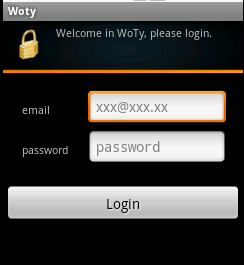
\includegraphics[scale=0.55]{images/login.png}
\caption{ Schermata di autenticazione }
\end{figure}
\end{center}


L'autenticazione al sistema permetterà l'attivazione del sistema di notifica che abiliterà le notifiche push inviate all'utente all'arrivo di nuove quest da svolgere. L'autenticazione non sarà più richiesta a meno che l'utente non effettui il log-out con la procedura descritta nel prossimo paragrafo.

\comment{\begin{center}
\begin{figure}[ht]
\centering
%\includegraphics[scale=0.55]{images/.png}
\caption{ Notifiche visualizzate all'arrivo di nuove quest }
\end{figure}
\end{center}}

\begin{center}
\begin{figure}[H]
\centering
\begin{tabular}{ m{5.5cm} m{5.5cm}}
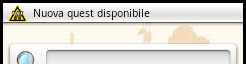
\includegraphics[scale=0.65]{images/notificaChiusa.png} & 
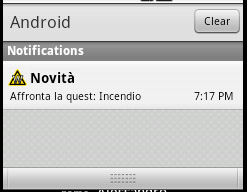
\includegraphics[scale=0.65]{images/notificaInApertura.png} \\
\end{tabular}
\caption{Arrivo e visualizzazione di una notifica}
\end{figure}
\end{center}

%\subsection{Sistema di notifica}
%L'autenticazione al sistema permetterà l'attivazione del sistema di notifica che abiliterà le notifiche push inviate all'utente %all'arrivo di nuove quest da svolgere.\\ Per non ricevere le notifiche l'utente potrà eseguire la normale procedura di disattivazione %delle notifiche per l'applicazione dalle opzioni del suo dispositivo.

\subsection{Menu delle opzioni}
	\label{optionsmenu}
	
\begin{center}
\begin{figure}[H]
\centering

\includegraphics[scale=0.70]{images/menu.png}
\caption{ Menu delle opzioni dell'applicazione }
\end{figure}
\end{center}	
	
Il menu delle opzioni dell'applicazione, attivabile con il pulsante ''menu'' del dispositivo permetterà le seguenti funzionalità:
\begin{itemize}
	\item \textbf{About}: provoca l'uscita della finestra di dialogo con le informazioni sull'applicazione. Da questa finestra l'utente potrà inoltre inviare le sue segnalazioni richiedendo assistenza all'indirizzo email del gruppo secondo le modalità descritte nel paragrafo \ref{assistenza}.

\begin{center}
\begin{figure}[H]
\centering
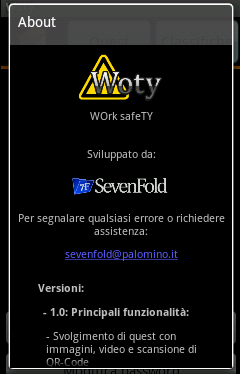
\includegraphics[scale=0.55]{images/about.png}
\caption{ Finestra delle informazioni }
\end{figure}
\end{center}	
	
	\item \textbf{Help}: provoca l'apertura della finestra di dialogo con la guida all'applicazione. La guida è divisa in sezioni riguardanti le varie funzionalità.
	
\begin{center}
\begin{figure}[H]
\centering
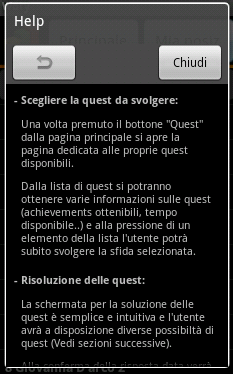
\includegraphics[scale=0.55]{images/help.png}
\caption{ Esempio di una finestra della guida all'uso dell'applicazione }
\end{figure}
\end{center}	
	
	\item \textbf{Log Out}: provoca il log-out dall'applicazione (vedi paragrafo precedente).	
\end{itemize}

\subsection{Schermata principale}

Una volta che l'utente ha effettuato l'autenticazione con successo si ritroverà nella schermata principale dell'applicazione, dove vengono visualizzati i dati dell'utente ed è possibile accedere alle sezioni che verranno spiegate nei paragrafi seguenti.

\begin{center}
\begin{figure}[H]
\centering
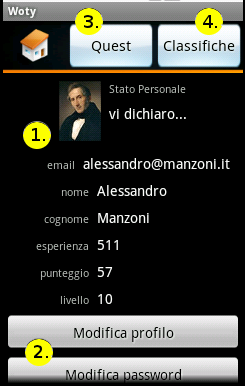
\includegraphics[scale=0.70]{images/home.png}
\caption{ Schermata principale Woty }
\end{figure}
\end{center}	

% magari mettere frecce sullo screenshot e poi scrivere qui sotto i numeri con la spiegazione se non è ridondante.
\begin{itemize}
	\item[\textbf{1.}] Avatar e dati personali
	\item[\textbf{2.}] Pulsanti per la modifica della password e dello stato personale
	\item[\textbf{3.}] Pulsante per l'accesso alle quest
	\item[\textbf{4.}] Pulsante per l'accesso alle classifiche del sistema
\end{itemize}


\subsection{Risoluzione delle quest}

Alla pressione del pulsante ''Quest'' dalla schermata principale si apre la schermata contenente la lista delle quest a disposizione, dalla quale l'utente può selezionare quelle che desidera svolgere. Nel caso in cui la lista sia vuota in quanto non vi sono al momento quest assegnate all'utente, sarà presente un pulsante con la quale l'utente potrà richiedere una quest.

\begin{center}
\begin{figure}[H]
\centering
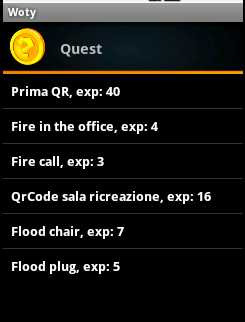
\includegraphics[scale=0.55]{images/pendinquests.png}
\caption{ Quest da svolgere }
\end{figure}
\end{center}

Alla selezione di una quest da parte dell'utente viene aperta la schermata dedicata all'esecuzione della stessa.

\begin{center}
\begin{figure}[H]
\centering
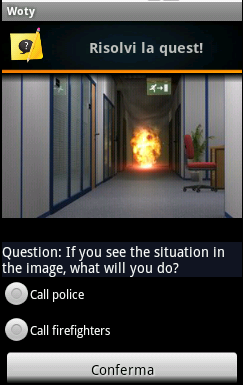
\includegraphics[scale=0.55]{images/solvequest.png}
\caption{ Esempio schermata svolgimento quest }
\end{figure}
\end{center}

Terminata l'esecuzione della quest l'utente si ritroverà alla schermata delle quest da svolgere e gli verrà notificato l'esito della quest precedente con un messaggio.

\subsection{Visione delle classifiche}

Alla pressione del pulsante ''Classifiche'' dalla schermata principale si apre la schermata di visualizzazione delle classifiche del sistema. In ogni schermata saranno visibili al massimo 20 elementi in classifica alla volta per limitare i dati in memoria nel dispositivo, ma sarà possibile spostarsi e visualizzare tutti i partecipanti con varie modalità.\\
La prima classifica che verrà proposta all'utente sarà quella a livello di dipartimento.
Il punteggio per ogni dipartimento viene calcolato sommando i punteggi degli utenti all'interno degli stessi.

\begin{center}
\begin{figure}[H]
\centering
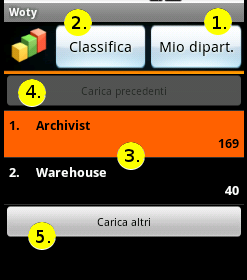
\includegraphics[scale=0.55]{images/workgroupsranks.png}
\caption{ Schermata delle classifica dei dipartimenti }
\end{figure}
\end{center}

\begin{itemize}
	\item[\textbf{1.}] Pulsante che porta alla posizione del dipartimento dell'utente (evidenziato in arancione).
	\item[\textbf{2.}] Pulsante che ritorna ai primi 20 dipartimenti in classifica.
	\item[\textbf{3.}] L'utente potrà visualizzare la classifica degli utenti interni a un dipartimento selezionandolo dalla classifica.
	\item[\textbf{4.}] Pulsante di richiesta dei precedenti dipartimenti presenti nella classifica.
	\item[\textbf{5.}] Pulsante di richiesta dei successivi dipartimenti presenti nella classifica.
\end{itemize}

Le classifiche interne ai dipartimenti sono strutturate in maniera analoga e mostrano i punteggi dei singoli utenti del sistema.

\begin{center}
\begin{figure}[H]
\centering
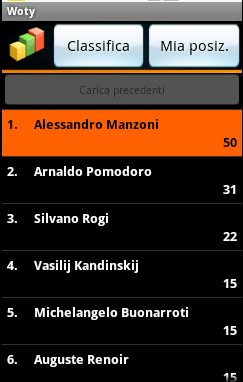
\includegraphics[scale=0.55]{images/usersranks.png}
\caption{ Schermata delle classifiche degli utenti}
\end{figure}
\end{center}

\begin{itemize}
	\item[\textbf{-}] L'utente potrà visualizzare le statistiche di un giocatore selezionandolo dalla classifica.
		
		\begin{center}
		\begin{figure}[H]
		\centering
		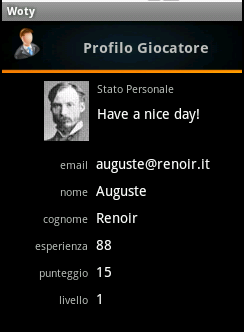
\includegraphics[scale=0.55]{images/playerprofile.png}
		\caption{ Visione del profilo di un utente in classifica }
		\end{figure}
		\end{center}

\end{itemize}



\subsection{Errori possibili}
Per qualsiasi tipo di errore, fare riferimento alla sezione \emph{''Come riportare problemi e malfunzionamenti''}.


\newpage

\section{Appendice}

	\subsection{Messaggi di errore e loro significato}
	
I principali messaggi di errore visualizzabili dall'applicazione sono:

\begin{itemize}

\item \textbf{Formato e-mail non valido}\\
Messaggio che indica che il formato dell'e-mail inserita dall'utente non è corretto

\item \textbf{Login non riuscito}\\
Messaggio che indica l'utente non ha inserito le credenziali corrette per l'autenticazione nel sistema

\item \textbf{Logout non disponibile}\\
Messaggio non può effettuare il logout a causa di problemi nel server o di connessione a internet.

\end{itemize}	
	

	\subsection{Glossario}
	\label{glossario}

\newLetter{A}

\newWord{Achievement}
Gratifica all'utente, archiviabile in uno storico, ottenuto in seguito al raggiungimento di determinati obiettivi.

\newWord{Android}
È un sistema operativo per dispositivi mobili costituito da uno stack software che include un sistema operativo di base, i middleware per le comunicazioni e le applicazioni di base.

\newWord{Android Market}
E' un negozio di software online sviluppato da Google per i dispositivi mobile che utilizzano il sistema operativo Android.

\newLetter{B}

\newWord{Badge}
Dall'inglese ''distintivo'', è un premio virtuale garantito ad un utente per aver completato un'azione all'interno di vincoli prestabiliti.

\newLetter{Q}

\comment{\newWord{QR-Code}
Codice a barre bidimensionale, composto da moduli neri disposti all'interno di uno schema di forma quadra. Viene impiegato per memorizzare informazioni generalmente destinate ad essere lette tramite smartphone.}

\newWord{Quest}
{Una quest è una una sfida che l'User dovrà compiere. Le tipologie di quest sono spiegate nella sezione 5.1 dell'appendice del documento \emph{AnalisiDeiRequisiti.pdf}.}

\newLetter{S}
\newWord{Sistema Operativo}
E' un particolare software, installato su un sistema di elaborazione, che funge da ''base'' al quale si appoggiano gli altri software, che dunque dovranno essere progettati in modo da essere riconosciuti e supportati da quel particolare sistema operativo.

\newWord{Smartphone}
In italiano telefonino intelligente, consiste in un dispositivo portatile che abbina funzionalità di telefono cellulare a quelle di gestione di dati personali.


\newLetter{W}
\newWord{Woty}
acronimo dal doppio significato WOrk safeTY, oppure Worker Of The Year.

\end{document}